\chapter{Listarakenteet}

Lista on tietorakenne, joka sisältää joukon alkioita tietyssä järjestyksessä.
Esimerkiksi $[3,7,2,5]$ on lista, jossa on neljä alkiota.
Tavoitteemme on, että voimme tehokkaasti lisätä ja poistaa listan alkioita.

Tämä luku käsittelee kaksi tapaa listan toteuttamiseen:

\begin{itemize}
\item \textbf{Taulukkolista}: Lista on toteutettu taulukkona,
jonka kokoa muutetaan tarvittaessa.
\item \textbf{Linkitetty lista}: Lista on toteutettu erillisinä solmuina,
jotka on linkitetty toisiinsa.
\end{itemize}

Molemmissa toteutuksissa on omat hyvät ja huonot puolensa,
joihin kiinnitämme huomiota luvun aikana.

\section{Taulukkolista}

Taulukko on tehokas perustietorakenne, joka soveltuu hyvin listan alustaksi.
Ainoa ongelma on, että taulukon koko on kiinteä: meidän täytyy päättää alussa,
montako alkiota taulukossa on, emmekä voi muuttaa kokoa myöhemmin.
Esimerkiksi seuraava koodi luo taulukon, jossa on 10 alkiota:

\begin{code}
int[] taulu = new int[10];
\end{code}

Kuinka voisimme luoda muuttuvan kokoisen listan taulukon avulla?
Ratkaisuna on, että varaamme taulukkoon \emph{ylimääräistä}
tilaa tuleville listan alkioille.
Tälla tavalla voimme luoda listan, joka pystyy laajentumaan.
Seuraavaksi käymme läpi kaksi toteutusta,
joista ensimmäisessä listan loppuun voi lisätä alkioita
ja toisessa sekä alkuun että loppuun voi lisätä alkioita.

\subsection{Lisääminen loppuun}

Ideana on säilyttää listaa taulukossa niin,
että tietty määrä taulukon ensimmäisiä alkioita on listan käytössä
ja loput alkiot on varattu tuleville alkioille.
Kuva \ref{fig:listau} näyttää esimerkin listan $[3,7,2,5]$ tallentamisesta taulukkoon.
Taulukossa on paikkoja kymmenelle alkiolle, ja niistä neljä on tällä hetkellä käytössä.
Kun listan loppuun lisätään uusi alkio 6, se mahtuu taulukkoon.
Tällä tavalla alkion lisääminen listaan vie vain $O(1)$ aikaa.

\begin{figure}
\center
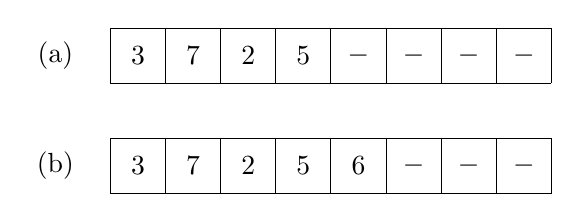
\begin{tikzpicture}[scale=0.7]
\begin{scope}
\draw (0,0) grid (8,1);
\node at (-1,0.5) {(a)};
\node at (0.5,0.5) {$3$};
\node at (1.5,0.5) {$7$};
\node at (2.5,0.5) {$2$};
\node at (3.5,0.5) {$5$};
\node at (4.5,0.5) {$-$};
\node at (5.5,0.5) {$-$};
\node at (6.5,0.5) {$-$};
\node at (7.5,0.5) {$-$};
\end{scope}
\begin{scope}[yshift=-2cm]
\draw (0,0) grid (8,1);
\node at (-1,0.5) {(b)};
\node at (0.5,0.5) {$3$};
\node at (1.5,0.5) {$7$};
\node at (2.5,0.5) {$2$};
\node at (3.5,0.5) {$5$};
\node at (4.5,0.5) {$6$};
\node at (5.5,0.5) {$-$};
\node at (6.5,0.5) {$-$};
\node at (7.5,0.5) {$-$};
\end{scope}
\end{tikzpicture}
\caption{(a) Lista $[3,7,2,5]$ tallennettuna taulukkoon. (b) Listan loppuun lisätään alkio 6.}
\label{fig:listau}
\end{figure}

Tässä on kuitenkin yksi ongelma: jossain vaiheessa koko taulukko
voi täyttyä eikä uusi listalle lisättävä alkio mahdu enää taulukkoon.
Kuva \ref{fig:lisuus} näyttää tällaisen tilanteen,
jossa uusi alkio 4 ei mahdu taulukkoon.
Tällöin meidän täytyy varata uusi suurempi taulukko ja
kopioida kaikki vanhan listan alkiot siihen.
Tämä on hidas operaatio, johon kuluu aikaa $O(n)$,
kun listalla on $n$ alkiota.
Olemme saaneet siis aikaan listan, johon on \emph{yleensä} nopeaa lisätä
alkioita, mutta välillä lisääminen viekin aikaa $O(n)$.

\begin{figure}
\center
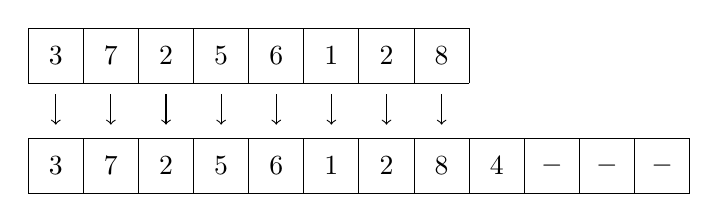
\begin{tikzpicture}[scale=0.7]
\begin{scope}
\draw (0,0) grid (8,1);
\node at (0.5,0.5) {$3$};
\node at (1.5,0.5) {$7$};
\node at (2.5,0.5) {$2$};
\node at (3.5,0.5) {$5$};
\node at (4.5,0.5) {$6$};
\node at (5.5,0.5) {$1$};
\node at (6.5,0.5) {$2$};
\node at (7.5,0.5) {$8$};
\foreach \x in {0,...,7} \draw[->] (\x+0.5,-0.2) -- (\x+0.5,-0.75);
\end{scope}
\begin{scope}[yshift=-2cm]
\draw (0,0) grid (12,1);
\node at (0.5,0.5) {$3$};
\node at (1.5,0.5) {$7$};
\node at (2.5,0.5) {$2$};
\node at (3.5,0.5) {$5$};
\node at (4.5,0.5) {$6$};
\node at (5.5,0.5) {$1$};
\node at (6.5,0.5) {$2$};
\node at (7.5,0.5) {$8$};
\node at (8.5,0.5) {$4$};
\node at (9.5,0.5) {$-$};
\node at (10.5,0.5) {$-$};
\node at (11.5,0.5) {$-$};
\end{scope}
\end{tikzpicture}
\caption{Taulukkoon ei mahdu enää uutta alkiota. Meidän täytyy varata uusi suurempi taulukko
ja kopioida vanhan taulukon sisältö sinne.}
\label{fig:lisuus}
\end{figure}

Jotta rakenne olisi käyttökelpoinen, meidän täytyy varmistaa,
että hidas $O(n)$-operaatio ei esiinny liian usein.
Tämä on mahdollista, kun varaamme reilusti suuremman uuden taulukon
aina silloin, kun vanha taulukko käy liian pieneksi.
Esimerkiksi voimme varata uuden taulukon niin,
että sen koko on kaksinkertainen vanhaan taulukkoon nähden.
Kun toimimme näin, jokaisen alkion lisääminen listalle vie
\emph{keskimäärin} vain $O(1)$ aikaa.

Voimme ajatella asian näin: jokainen listalle lisättävä alkio
maksaa pääsy\-maksuna kolme euroa.
Tästä yksi euro menee listalle liittymiseen ja kaksi euroa jäävät säästöön.
Sitten kun aikanaan listalle täytyy varata suurempi taulukko,
jokainen viime erässä lisätty alkio maksaa yhden euron omasta siirrostaan
ja yhden euron aiemmin lisätyn alkion siirrosta.
Koska taulukon koko kaksinkertaistuu joka vaiheessa,
kolmen euron kiinteä pääsymaksu riittää siihen, että kaikki tulevat
siirrot saadaan kustannettua.

Miksi sitten emme voisi varata heti aluksi niin suurta taulukkoa,
että lopullinen lista mahtuisi siihen varmasti?
Tässä tulisi ongelmaksi, että listamme tuhlaisi paljon muistia.
Ohjelmassa saattaa olla samaan aikaan käytössä monia listoja,
ja haluamme, että listan varaama taulukko on samaa kokoluokkaa
kuin listan todellinen sisältö.

\subsection{Lisääminen alkuun ja loppuun}

\subsection{Javan rakenteet}

Javassa \texttt{ArrayList}-rakenne toteuttaa taulukkolistan,
jossa on nopeaa lisätä alkio loppuun sekä poistaa alkio lopusta.
Esimerkiksi seuraava koodi luo listan, lisää siihen alkiot
1, 2 ja 3 ja tulostaa listan sisällön.
Sitten koodi poistaa listan viimeisen alkion ja
tulostaa uudestaan listan sisällön.

\begin{code}
ArrayList<Integer> lista = new ArrayList<>();
lista.add(1);
lista.add(2);
lista.add(3);
System.out.println(lista); // [1, 2, 3]
lista.remove(2);
System.out.println(lista); // [1, 2]
\end{code}

Metodit \texttt{add} ja \texttt{remove}
toimivat keskimäärin ajassa $O(1)$,
joten voimme muuttaa tehokkaasti listaa sen lopusta.
Lisäksi koska lista on tallennetu taulukkona,
voimme tehokkaasti hakea tietyssä kohdassa olevan alkion
ja muuttaa tietyssä kohdassa olevaa alkiota
metodeilla \texttt{get} ja \texttt{set}.

Javassa on myös \texttt{ArrayDeque}-rakenne,
joka toteuttaa taulukkolistan, johon voi tehdä tehokkaita
lisäyksiä ja poistoja sekä alussa että lopussa.
Seuraava koodi esittelee rakenteen käyttämistä:

\begin{code}
ArrayDeque<Integer> lista = new ArrayDeque<>();
lista.addLast(1);
lista.addFirst(2);
lista.addLast(3);
System.out.println(lista); // [2, 1, 3]
lista.removeFirst();
System.out.println(lista); // [1, 3]
\end{code}

\texttt{ArrayDeque} sisältää metodit \texttt{getFirst} ja
\texttt{getLast}, joiden avulla voimme hakea listan
ensimmäisen ja viimeisen alkion.
Kuitenkaan rakenteessa ei ole yleistä metodia \texttt{get},
joten emme pysty hakemaan muita listalla olevia alkioita.


\section{Linkitetty lista}

\subsection{\texttt{LinkedList}-rakenne}
